% !TeX spellcheck = en_US
\documentclass[useAMS,usenatbib,referee]{biom}
\newcommand{\mE}{\ensuremath{\mathbb E}}
\newcommand{\mP}{\ensuremath{\mathbb P}}
\newcommand{\mR}{\ensuremath{\mathbb R}}
\usepackage{amsthm}
\theoremstyle{plain}
\newtheorem*{proposition*}{Proposition 6.1}
\newtheorem{ex}{Example}[section]
\newtheorem{cor}{Corollary}[section]
\usepackage{hyperref}
\usepackage{units}
%%\usepackage{multirow}
\usepackage{amsmath}
%\usepackage{amssymb}
%\usepackage{cancel}
\usepackage{graphicx}
%\PassOptionsToPackage{normalem}{ulem}
%\usepackage{ulem}
%\usepackage{endrotfloat}
\usepackage{amsfonts}       % blackboard math symbols
\usepackage{nicefrac}       % compact symbols for 1/2, etc.
\usepackage{microtype}      % microtypography
%\usepackage{lipsum}

\usepackage{xcolor}

\setcounter{secnumdepth}{3}

\usepackage{soul} % for strike out 
\newcommand{\ijcomm}[1]{\textcolor{red}{IJ:#1}}
\newcommand{\ijadd}[1]{\textcolor{red}{#1}}
\newcommand{\ijdel}[1]{\textcolor{red}{\st{#1}}}

\newcommand{\comment}[1]{}
\usepackage{soul} % for strike out 
\newcommand{\rhcomm}[1]{\textcolor{blue}{rh:#1}}
\newcommand{\rhadd}[1]{\textcolor{blue}{#1}}
\newcommand{\rhdel}[1]{\textcolor{blue}{\st{#1}}}

\newcommand{\btheta}{{\pmb \theta}}

%\def\bSig\mathbf{\Sigma}
%\newcommand{\VS}{V\&S}
%\newcommand{\tr}{\mbox{tr}}

\title{Supplementary material: Quantifying replicability and consistency in systematic reviews}

\author{
	Iman Jaljuli\emailx{jaljuli.iman@gmail.com} \\
	Department of Statistics and Operations Research, Tel-Aviv University, Tel-Aviv, Israel.
	\and
	Yoav Benjamini\emailx{ybenja@gmail.com} \\
	Department of Statistics and Operations Research, Tel-Aviv University, Tel-Aviv, Israel.
	\and
	Liat Shenhav\emailx{liashenhav@gmail.com} \\	
	Department of Computer Science, University of California Los Angeles, Los Angeles, CA, USA.
	\and
	Orestis A. Panagiotou\emailx{orestis\_panagiotou@brown.edu} \\	
	Department of Health Services, Policy \& Practice, Brown University, USA.
	\and
	Ruth Heller\emailx{ruheller@gmail.com} \\
	Department of Statistics and Operations Research, Tel-Aviv University, Tel-Aviv, Israel.}




\begin{document}
	
	\date{{\it Received XXX} 201X. {\it Revised XXX} 201X.  {\it
			Accepted XX} 201X.}
	
	\pagerange{\pageref{firstpage}--\pageref{lastpage}} 
	\volume{XX}
	\pubyear{2019}
	\artmonth{July}
	
	\doi{10.1111/j.1541-0420.2005.00454.xX}
	
	%  This label and the label ``lastpage'' are used by the \pagerange
	%  command above to give the page range for the article.  You may have 
	%  to process the document twice to get this to match up with what you 
	%  expect.  When using the referee option, this will not count the pages
	%  with tables and figures.  
	
	\label{firstpage}
	
	
	
	\maketitle		
	
	
	
	
	\section{Simulations}\label{sec-simulation}
	
	
	\subsection{Simulation settings}	
	
	
	For study $i\in \{1,\ldots,n\}$, the estimated effect size, $\hat \theta_i$, is sampled from the normal distribution with mean $\theta_i$ and standard deviation $SE_i = \sqrt{1/n_{Ci}+1/n_{Ti}}$, where $n_{Ci}$ and $n_{Ti}$ are the control and treatment group sizes, respectively. 
	We examined a wide range of values for $(\theta_1,\ldots, \theta_n)$, $n$, and $\{ (n_{Ci}, n_{Ti}): i=1,\ldots, n\}$. 
	
	In the paper, we displayed results for $n=8$, with unequal group sizes as follows: $ \left\lbrace 22, 210,  26, 192,  60,  38,  53,  15\right\rbrace $ for the control groups and  $ \left\lbrace 22, 121,  24, 187,  31,  53,  49,  16\right\rbrace $ for the treatment groups (these values are similar to those in the example detailed in Figure 8). 
	Simulations for other variations of $n=4,8,20$ with unequal samples sizes or equal  ( $\{ n_{Ci} = n_{Ti} = 25 \; \forall i=1,\ldots, n\}$) are shown in figures \ref{fig-sim2_extensions1} and \ref{fig-sim2_extensions2}
	
	\begin{figure}[htpb]
		\centering
		%	\includegraphics[width=0.9\textwidth]{sim2_new.pdf} 
		\includegraphics[page = 2, width=0.9\textwidth]{sim2_all.pdf} 
		\caption{ Each panel shows the results of a simulation similar to figure 2 in the body of the paper. The different panels differentiate by the number of studies $N$ and whether the group sizes are equal on not (detailed in the panel title).
			%Rejection rate as function of the strength of the fixed effects vector characterized by $\mu$. The effects vector $\left( \theta_1,\theta_2, \dots ,\theta_8\right) $ is  indicated at the top of each column. The null hypotheses  examined are: the RE meta-analysis null  (dashed), the global null $H^{1/n}$ (row 1), the minimal replicability null $H^{2/n}$ (row 2), $H^{3/n}$ (row 3), no lack of consistency (row 4). Except for the RE meta-analysis null, the test statistics  use products of  truncated $p$-values at most: 0.05 (solid red); 0.5 (solid green); or 1 (solid blue). The horizontal solid line is the 0.05 significance level of the test. The effect estimates $\hat{\theta}_j$ are sampled from the normal distribution with mean $\theta_j$ and standard deviation $SE_j$.   The replicability null hypothesis, $H^{2/n}$, is true in the first column  and false otherwise. The inconsistent setting is in the left column. 
		}\label{fig-sim2_extensions1}
	\end{figure}
	
	
	\begin{figure}[htpb]
		\centering
		\includegraphics[page = 3, width=0.9\textwidth]{sim2_all.pdf} 
		\caption{ Each panel shows the results of a simulation similar to figure 2 in the body of the paper. The different panels differentiate by the number of studies $N$ and whether the group sizes are equal on not (detailed in the panel title).
		}\label{fig-sim2_extensions2}
	\end{figure}
	
	
	
	
	\begin{figure}[htpb]
		\centering
		\includegraphics[page = 2, width=0.9\textwidth, height= 0.46\textheight]{sim4_all.pdf} 
		\caption{  Each panel shows the results of a simulation similar to figure 3 in the body of the paper. The different panels differentiate by the number of studies $N$ and whether the group sizes are equal on not (detailed in the panel title).
			%Rejection rate versus the number of nonnull studies with a common treatment effect, with the RE meta-analysis test (dashed) or with the no replicability test of $H^{2/n}$ (solid).    The curves with: circles, triangles, and squares, have treatment effect  value of one, two, and three, respectively.  The replicability null hypothesis, $H^{2/n}$,  is true when the number of studies is zero or one, and false otherwise. The horizontal solid line is the 0.05 significance  level of  the test. The product of truncated $p$-values are truncated at $t=0.05$. 
		}\label{fig-simFE_extensions}
	\end{figure}
	
	
	
	Figure \ref{fig-sim3_extensions} shows results for the random effects settings in figure 4 in the body of the paper. Here we show for $N=4,8,20$ with unequal samples sizes ( like in fig.~\ref{fig-sim2_extensions1}), or with equal group sizes ( $\{ n_{Ci} = n_{Ti} = 25 \; \forall i=1,\ldots, n\}$). 
	
	
	
	
	
	
	\begin{figure}[htpb]
		\centering
		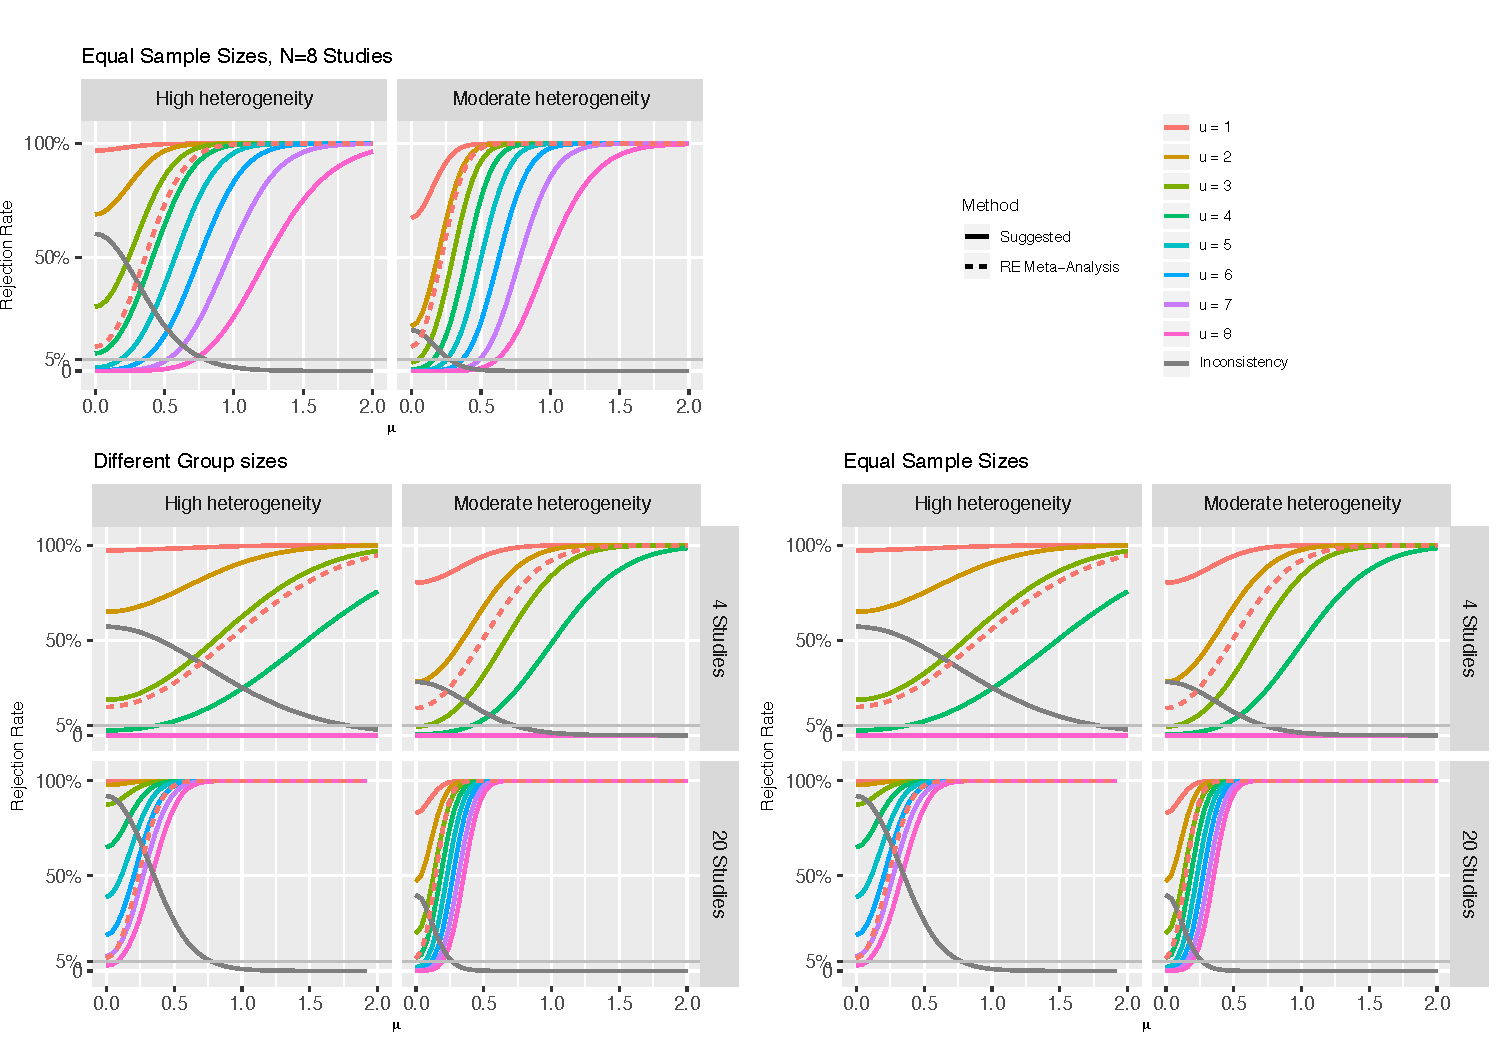
\includegraphics[width=\textwidth, height= 0.55\textheight]{sim3B_all.pdf} 
		\caption{ Each panel shows the results of a simulation similar to figure 3 in the body of the paper. The different panels differentiate by the number of studies $N$ and whether the group sizes are equal on not (detailed in the panel title).
			%Rejection rate as a function of the overall treatment effect $\mu$ in data generated according to the RE model. The hypotheses tests examined are: the RE Meta-analysis null that $\mu=0$ (dashed), and  $H^{u/n}$ for $u=1,\ldots,8$ (solid). For study $j=1,\ldots,8$, treatment effect estimate $\hat \theta_j$ is sampled form the normal distribution with mean $
			%	\theta_j$ and standard deviation $SE_j$. The treatment effect $
			%	\theta_j$ is itself sampled independently from the normal distribution with mean $\mu$ and standard deviation $\tau$. The value of $\tau$ is chosen so the estimated heterogeneity is around 70\% in the left panel, and around 50\% in the right panel. The product of truncated $p$-values are truncated at $t=0.05$. 
		}\label{fig-sim3_extensions}
	\end{figure}
	
	
	
	
	
	
	
	\section{ Replicability-analysis: Assuming common effect }\label{sec-rvalueFE}
	
	
	%	\begin{proposition*}
	%		Let $Z=\hat \theta/\widehat{SE}$ be the fixed-effects meta-analysis test statistic, with meta-analysis $p$-value $p = 2\min(p^R, p^L)$, where $p^L = \Phi(Z)$ and $p^R =  1-\Phi(Z)$.  Let $r(u), r^L (u), r^R (u)$ be the $u$ out of $N$ $r$-values for $u\in \{2,\ldots,n \}$, as defined in this section. Then $p<r(u)$, and moreover,  if $Z<0$, $p^L<r^L(u)$, and if $Z>0$, $p^R<r^R(u)$. 
	%	\end{proposition*}
	
	
	
	
	
	
	\subsection*{Proof of proposition 6:}
	%	\begin{proof}
	%	\subsubsection*{proof}
	Let $Z_v$, $\hat \theta_v$, and $SE_v$ be the fixed-effect meta-analysis test statistic, estimated effect, and SE, respectively, for the intersection hypotheses indexed by $v\in \Pi(n-u+1)$.
	%The following two algebraic identities will be used: 
	%\begin{eqnarray}
	%&&\sum_{v\in \Pi(n-u+1)} \frac{z_v}{SE_v}  =\binom{n-1}{n-u}\sum_{i=1}^n\frac{\hat \theta_i}{SE_i} \label{eq-pf1} \\
	%&& \sum_{v\in \Pi(n-u+1)} \frac{1}{SE^2_v}  =\binom{n-1}{n-u}\sum_{i=1}^n\frac{1}{SE^2_i}  = \binom{n-1}{n-u}\frac{1}{SE^2}  \label{eq-pf2} 
	%\end{eqnarray}
	Since $\sum_{v\in \Pi(n-u+1)} \frac{z_v}{SE_v}  =\binom{n-1}{n-u}\sum_{i=1}^n\frac{\hat \theta_i}{SE_i}$, the meta-analysis test statistic can be expressed in terms of $(z_v, SE_v)$, $v\in \Pi(n-u+1)$:
	\begin{equation}
	Z = \frac1{\binom{n-1}{n-u}}\sum_{v\in \Pi(n-u+1)} \frac{z_v}{SE_v}SE \label{eq-pf1}
	\end{equation}
	Let $v^* = \arg \max_{v\in\Pi(n-u+1)} Z_v$. By definition,  $r^L = \Phi(Z_{v^{*}})$. We shall show that if $Z<0$, $p^L<r^L$ and $\min(p^L,p^R)< min(r^L,r^R)$. 
	Clearly, $p^L<0.5$ since 
	$Z<0$. Therefore, the result follows by showing that $p^L<r^L$ and $r^R>0.5$.   
	
	
	We start by showing that $p^L<r^L$.  If $Z_{v^*}>0$, then by definition $r^L>0.5$ and therefore  it follows that $P^L<r^L$.  If $Z_{v^*}<0$ then 
	\begin{eqnarray}
	Z\leq  \frac{Z_{v^*}}{\binom{n-1}{n-u}}\sum_{v\in \Pi(n-u+1)} \frac{SE}{SE_v}\leq  \frac{Z_{v^*}}{\binom{n-1}{n-u}}\sum_{v\in \Pi(n-u+1)} \frac{SE^2}{SE^2_v} = Z_{v^*}, \nonumber
	\end{eqnarray}
	where the first inequality follows from \eqref{eq-pf1} and the definition of $v^*$, the second inequality follows since $SE/SE_v<1$ for all $v\in\Pi(n-u+1)$, and the last equality follows since $$\sum_{v\in \Pi(n-u+1)} \frac{1}{SE^2_v}  =\binom{n-1}{n-u}\sum_{i=1}^n\frac{1}{SE^2_i}  = \binom{n-1}{n-u}\frac{1}{SE^2}. $$ 
	Since $Z\leq Z_{v^*}$ it thus follows that $p^L<r^L$. 
	
	Next, we show that $r^R>0.5$. By definition,  $r^R = 1- \Phi(\min_{v\in\Pi(n-u+1)} Z_v)$. Since $Z<0$ and  
	$$\frac{\min_{v\in\Pi(n-u+1)} Z_v}{\binom{n-1}{n-u}}\sum_{v\in \Pi(n-u+1)} \frac{SE}{SE_v}<Z, $$ it follows that $\min_{v\in\Pi(n-u+1)} Z_v<0$ and therefore that $r^R>0.5$. 
	
	
	
	Therefore, if $Z<0$ we have $p^R<r^R$ and $\min(p^L,p^R)<\min(r^L,r^R)$. 
	Similar arguments show that if $Z>0$, $p^R<r^R$ and  $\min(p^L,p^R)<\min(r^L,r^R)$. It thus follows that $p<r$. 
	%	\end{proof}
	
	\begin{remark}
		The property that, with probability one,  the global null $p$-value is smaller than the $r$-value, is not satisfied with popular combining functions such as Fisher, Simes, and Bonferroni. 
		For example, if $p_{(1)}\leq \ldots \leq p_{(n)}$ are the ordered $p$-values, then the Bonferroni meta-analysis $p$-value is $n\times p_{(1)}$, its $r$-value for $u=2$ is $(n-1)\times p_{(2)}$, and $Pr \left(n\times p_{(1)}<(n-1)\times p_{(2)}\right)>0. $ 
	\end{remark}
	
	
\end{document}


